% 文件类型:中文文章
% 编码形式:UTF8
% ctexart:调用CTEX宏包,支持中文
% fontset = none:不使用预设字体
\documentclass[UTF8]{ctexart}

% ===============================================页面设置=============================================== %
% 设置页面大小
\usepackage{geometry}
\geometry{a4paper} % 设置版面为A4纸张
\geometry{top=1in, bottom=1in, left=1in, right=1in}

% 设置页眉页脚相关
% \usepackage{CJK}
\usepackage{lastpage} % 显示页数使用
\usepackage{fancyhdr}
\pagestyle{fancy} % 设置页眉页脚
\fancyhf{} % 清除所有页眉页脚            
\lhead{电流采样}   %页眉左侧显示页数                 
\chead{page \thepage\ of \pageref{LastPage}} %页眉中
\rhead{采样电阻方案} %章节信息                       
\cfoot{\thepage} %当前页,记得调用前文提到的宏包                
\rfoot{页脚左}%                                                       
\lfoot{页脚右}
\renewcommand{\headrulewidth}{0.1mm} %页眉线宽,设为0可以去页眉线
\renewcommand{\footrulewidth}{0.1mm} %页脚线宽,设为0可以去页眉线
% 设置页眉页脚相关间距
\setlength{\voffset}{-10mm} % 调整页面垂直移动参数                       
\setlength{\topmargin}{0mm} % 上边距
\setlength{\headheight}{5mm} % 页眉高度
\setlength{\headsep}{5mm} % 页眉与正文间距
\setlength{\footskip}{5mm} % 正文与页脚基线间距

% ===============================================文章格式=============================================== %
% 设置文章主题字体,默认中文为宋体
% \usepackage{xeCJK}
% \usepackage{fontspec} % 字体包
% \setCJKmainfont{FangSong} % 设置中文主题字体
% \setmainfont{TeX Gyre Termes} % 设置英文主题字体

% 行间距设置
\usepackage{setspace}
\setstretch{1.5} % 行间距1.5倍

% 标题设置
\usepackage{titlesec}
% \titleformat{command}{format}{label}{sep}{before-code}
% command:指定格式使用地方,此时为一级标题
% shape:格式
% format:左对齐raggedright、大标题、加粗显示
% label:设置格式
% sep:设置间距
% before-code:保持空格
\titleformat{\section}[block]{\raggedright\Large\bfseries}{\thesection}{1em}{}
\titleformat{\subsection}[block]{\raggedright\large\bfseries}{\thesubsection}{1em}{}
\titleformat{\subsubsection}[block]{\raggedright\normalfont\bfseries}{\thesubsubsection}{1em}{}

% ===============================================图片设置=============================================== %
%图片引用包含包
\usepackage{graphicx} 
\usepackage{float}
\usepackage{subfigure}
\usepackage{caption}
\captionsetup[figure]{name={Fig.},labelsep=space} % 设置图片数字后为空格,如Figx.x  xxx
\captionsetup{font={small,stretch=1.0}} % 图注字体大小设置

% ===============================================数学公式=============================================== %
\usepackage{amsmath}
\usepackage{lmodern} % 消除字体差异引起编译器报Warning
\usepackage{newtxmath} % 实现粗体字母数字导入
\numberwithin{equation}{section} % 设置公式编号:章节 + 序号
\numberwithin{figure}{section}

% ===============================================文章编写=============================================== %
\begin{document}

% 标题
\title{\zihao{-2} 采样电阻电流测量方案分析}
\author{Peilong Zhang}
\date{} % 日期参数为空,不显示日期
\maketitle
\thispagestyle{fancy} % 标题页也使用页眉页脚格式


% ===============================================第一章节=============================================== %
\section{简介}
\subsection{电流产生}

    在物理学上,带电粒子的定向运动形成电流,电流强度的计算公式为:
    \begin{equation}
        I = \frac{\Delta q}{\Delta t}
        \label{e1.1}
    \end{equation}
    \par % \par或插入空行,插入新的段落
    式(\ref{e1.1})从一个宏观的角度给出了电流强度的计算方法,也表明了形成电流的条件之一就是需要有随时间变化的电荷。对于
    导体而言,导体中的正电荷为金属原子核,原子核按照一定的规律紧密排列,构成宏观上的导体,不会随意运动;因此导体中可以
    自由移动的电荷为自由电子,自由电子具有以下几种运动方式:
    
    1)在有外加电场的情况下,受到电场力的作用,自由电子沿电场梯度的负方向定向移动,由式(\ref{e1.1})即可认为导体中形成了
    可以测得电流;
    
    2)无规则热运动,当导体处于绝对零度以上时,粒子吸收热进行无规则热运动,电子也不例外。无规则热运动的方向、速度均是随
    机的,从统计学意义上认为导体中所有电子的热运动速度矢量叠加后为0,因此可认为电子的无规则热运动并不会引起导体中宏观电
    流的产生。无规则热运动的影响会在后面进行介绍。

    真空中电子在恒定电场的作用下做匀加速直线运动,表现为速度越来越快;但在导体中由于晶格的存在,电子和晶格发生碰撞,运动
    受到阻碍,不再呈现匀加速直线运动。导体对电子运动的阻碍能力宏观上表现为导体电阻\textit{R},采用欧姆定律描述:
    \begin{equation}
        \Delta U = I \times R
        \label{e1.2}
    \end{equation}
    
    式(\ref{e1.2})中,$\Delta U$是导体两端的电压降,\textit{I}为流经导体的电流,为方便解释此处认为\textit{I}是一个恒定
    量。采用电场强度\textbf{\emph{E}}和电流密度\textbf{\emph{J}}、电导参数$\sigma$描述欧姆定律:
    \begin{equation}
        \textbf{\emph{E}} = \sigma \textbf{\emph{J}}
        \label{e1.3}
    \end{equation}

    式(\ref{e1.3})适用于均匀导体,导体不同方向上的电导率一致;而对于不同方向上电导率不一致即\textbf{各向异性}物质,采用
    电导张量描述该特性。电导张量是一般是$3 \times 3$形式的矩阵,如式(\ref{e1.4})所示:
    \begin{equation}
        \sigma = 
        \begin{bmatrix} % 插入矩阵
            \sigma_{11} &   \sigma_{12} &   \sigma_{13} \\ % \\表示一次换行或空行
            \sigma_{21} &   \sigma_{22} &   \sigma_{23} \\
            \sigma_{31} &   \sigma_{32} &   \sigma_{33}  % 最后一行不需要空行   
        \end{bmatrix}
        \label{e1.4}
    \end{equation}

    此时电流密度的表达式为:
    \begin{equation}
        \textbf{\emph{J}} = \sum_{i=1}^{3}\sigma_{ij} {\textbf{\emph{E}}_j}
        \label{e1.5}
    \end{equation}

    式(\ref{e1.5})反映了各项异性带来的影响,如对于$\textbf{\emph{J}}_1$方向上的电流密度,受到三个方向上的电场强度的影响。
    对于各向同性的导体,式(\ref{e1.5})中电导矩阵的对角线元素均为导体电导$\sigma_0$,其余元素均为0,式(\ref{e1.5})退化为式
    (\ref{e1.4}),即认为此时电导是一个标量。

\subsection{电阻采样基本原理}
    由式(\ref{e1.2}),导体内部电流由外加电场引起,电场在一定长度的导体两端表现为电压降$\Delta U$,可通过测量电阻两端的电压降,
    再除以导体电阻即可得到流过电阻的电流。用于测量电流的电阻一般称为采样电阻。


% ===============================================第二章节=============================================== %
\section{采样电阻测量电流方案设计}
\subsection{总体方案}
    采用采样电阻测量电流时,总体方案如图\ref{f2.1}所示。
    \begin{figure}[htbp] % htbp表示图片浮动
        \centering
        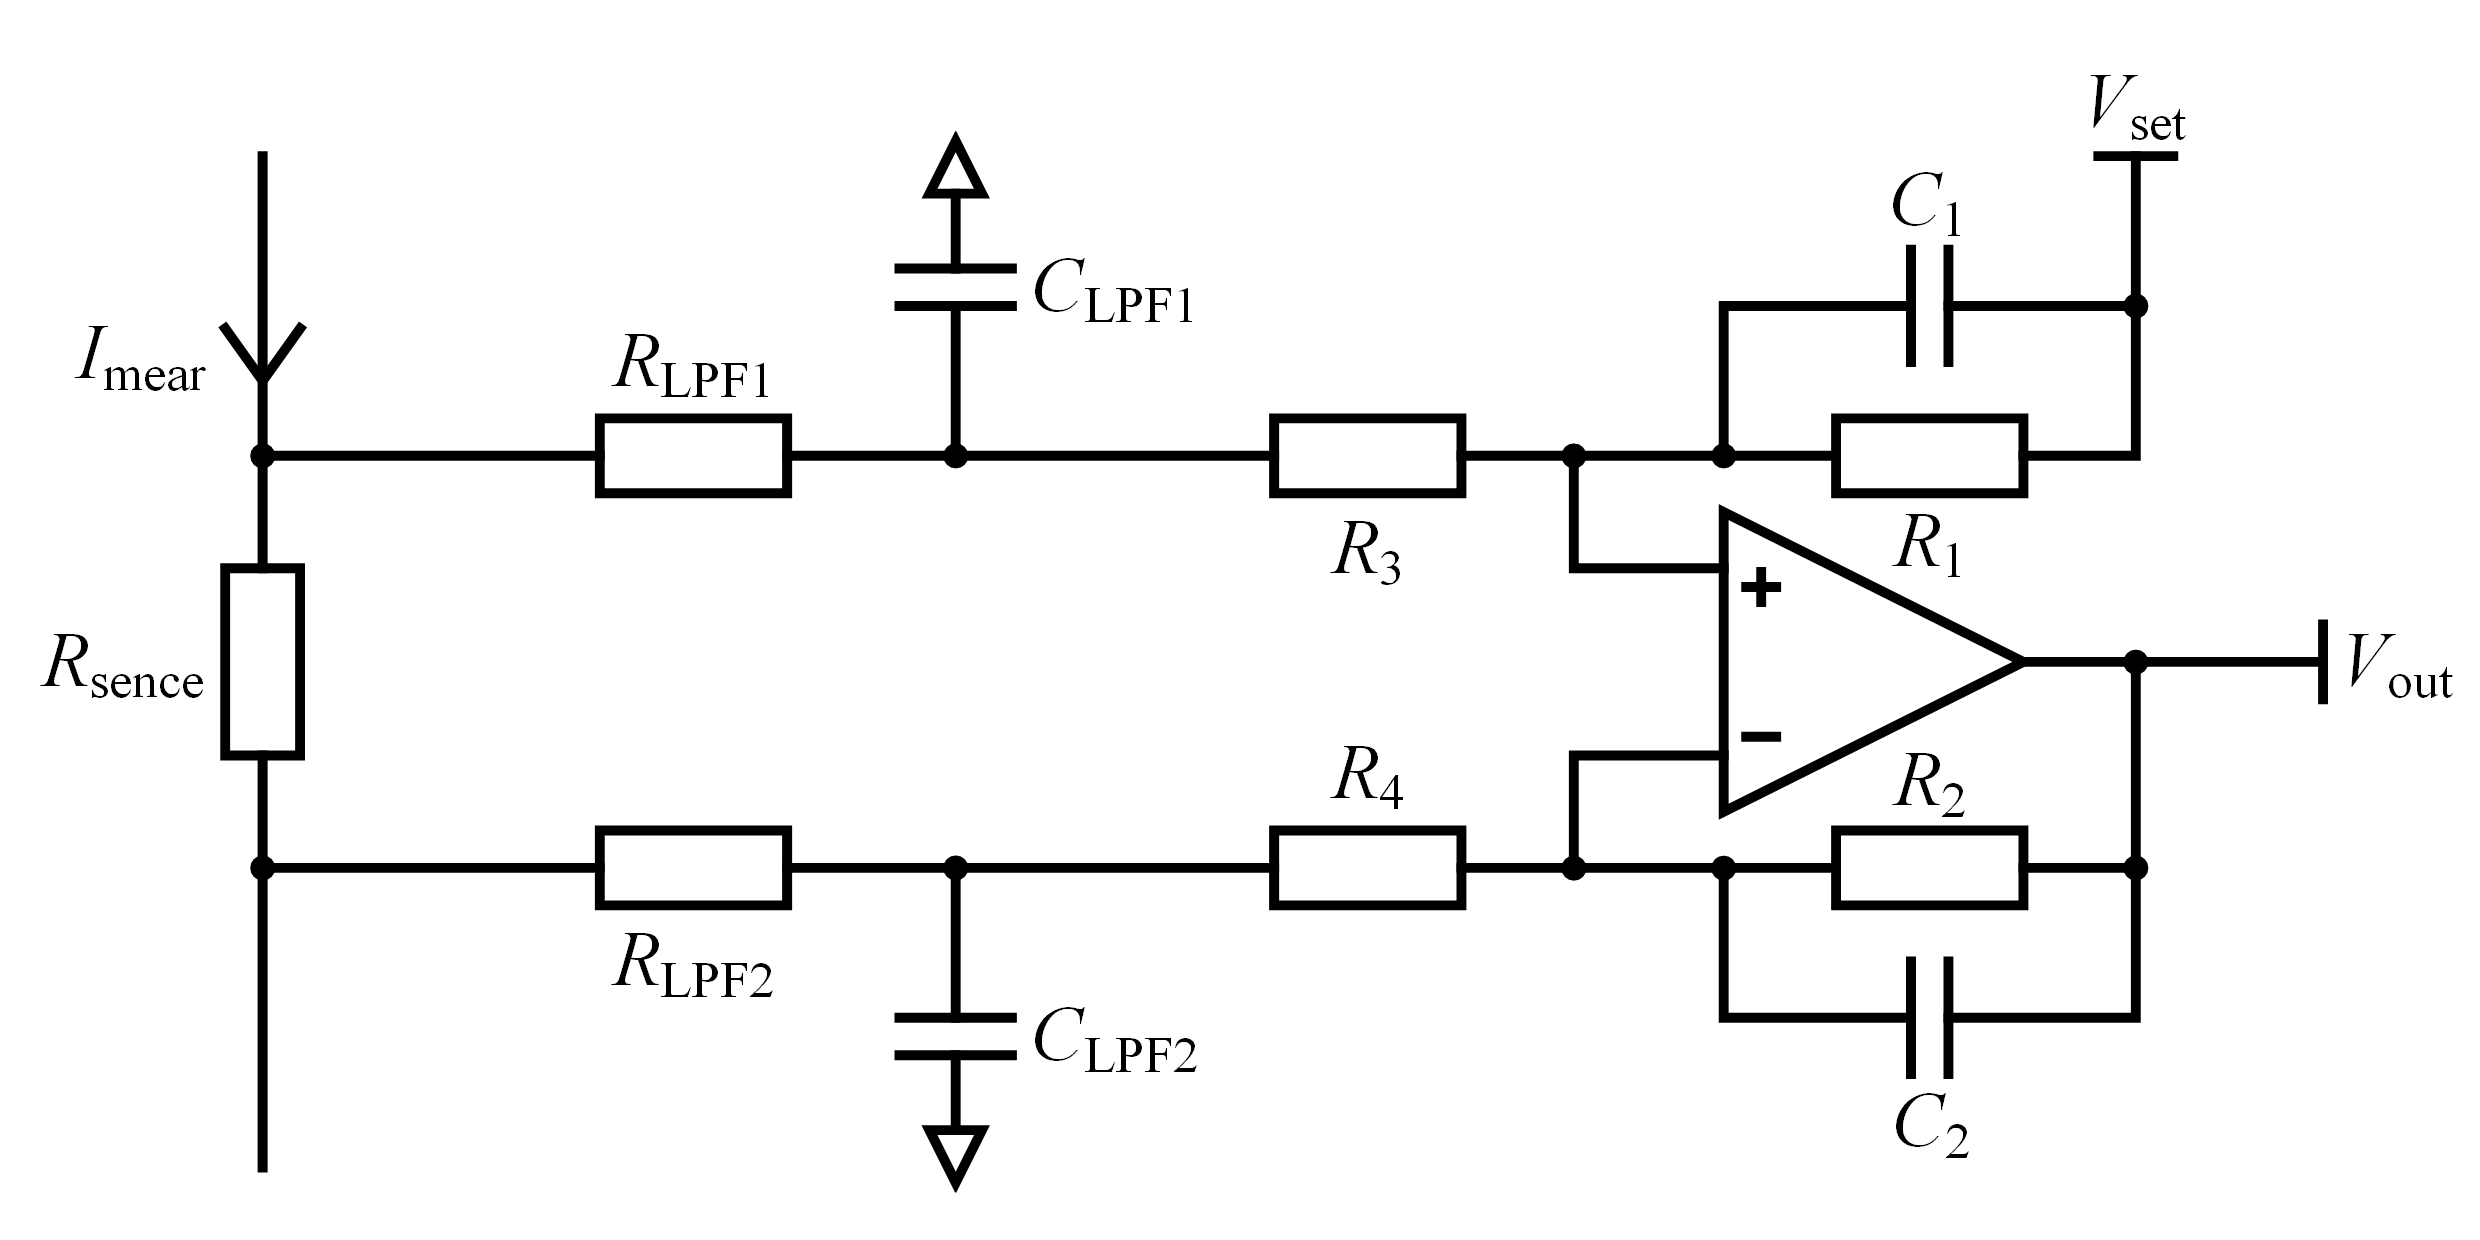
\includegraphics[scale = 1.4]{picture/1_resistor_sample.png}
        \caption{\space\ 采样电阻测量电流方案示意图} % 插入一个空格
        \label{f2.1}
    \end{figure}

    如图\ref{f2.1}所示,方案一般分为两部分:

    1)采样电阻本体$R_{\rm sense}$,为被测量电流$I_{\rm mear}$提供流通路径,在电阻两端形成电压降,实现电流到电压的转换。

    2)后级放大滤波,考虑到电阻功耗和发热等因素,采样电阻两端的电压降$\Delta U$一般较小,在某型情况下采样电阻输出的电压对测量地
    电位具有较高的共模分量,不适合直接送入ADC采样,因此在采样电阻输出到ADC输入端会增加一级或多级运放电路,用于对电阻电压进行放大、
    滤波、共模衰减等操作,用于适配ADC采样需求。

    在图\ref{f2.1}中,$R_{\rm LFP1}$与$C_{\rm LFP1}$、$R_{\rm LFP2}$与$C_{\rm LFP2}$构成两对一阶RC低通滤波器,可对差模和共
    模电压进行滤波;后级运放与$R_1 \sim R_4$、$C_1 \sim C_2$构成一级差分转单端放大电路(或减法电路),且通过配置RC并联阻抗的位
    置,兼顾放大和滤波。通过良好地匹配$R_1$和$R_2$、$R_3$与$R_4$,可实现较高的共模抑制比(Common-Mode Rejection Ratio,CMRR)
    ,减小采样电阻上共模电压对输出的影响。$V_{\rm set}$用于设定输出电压相对于地电位的偏置电平,使得该电路具备双向电流测量能力。
    % \sim为符号~

\subsection{采样电阻位置}
    由图\ref{f2.1},测量方案只给了电流、电阻等信息,只知道测量电阻输出的差分电压$\Delta U$,不知道电阻两端电压相对于功率地或信号
    地的电压。根据采样电阻与电源、负载的相对位置关系,电流采样可分为高侧电流采样和低侧电流采样,具体见图\ref{f2.2}.

    \begin{figure}[htb]
        \centering
        \subfigure[高侧电流采样]{
            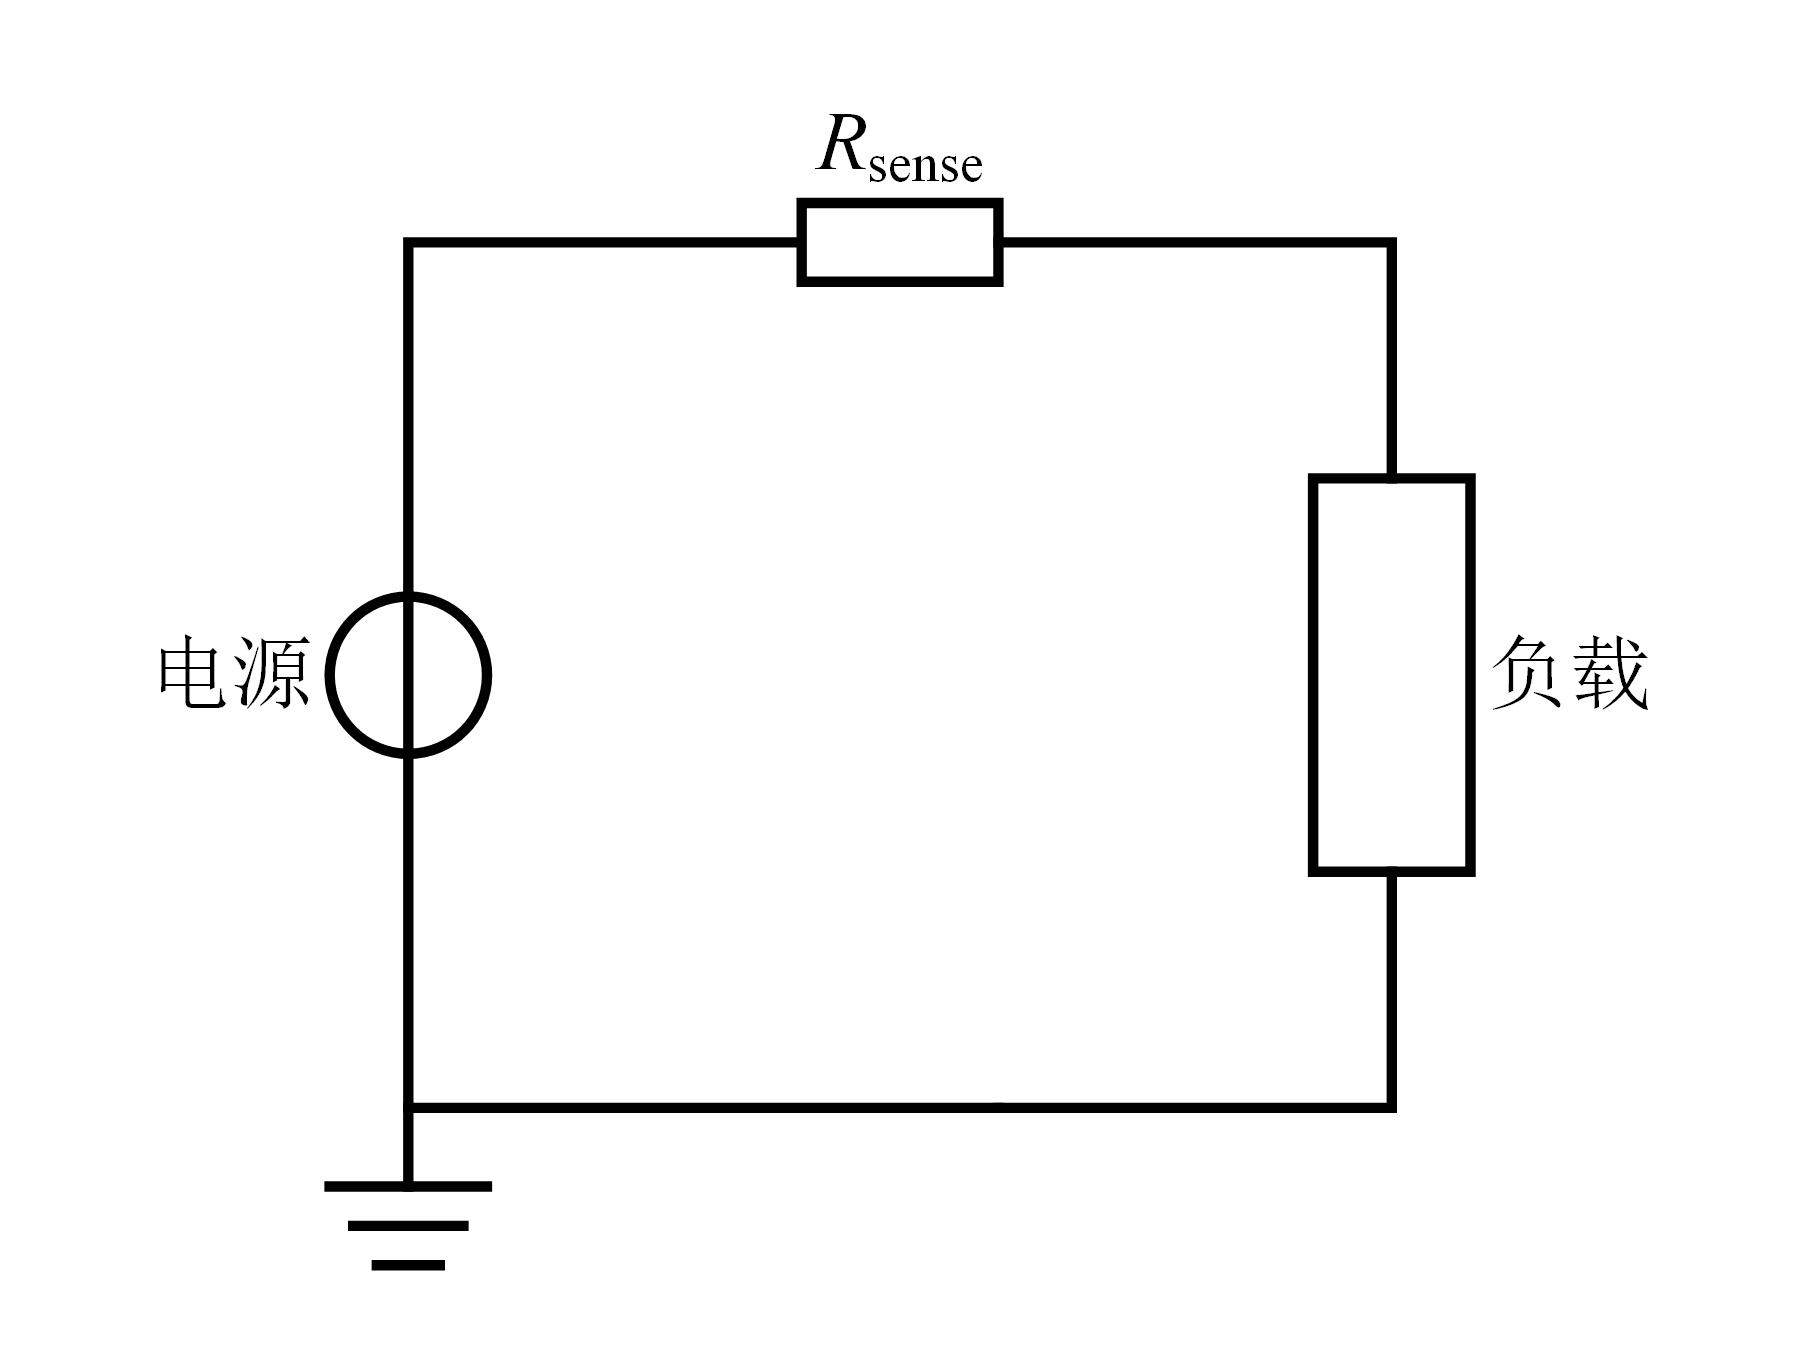
\includegraphics[scale=1.0]{picture/2_resistor_location_high.png}
            \label{f2.2:sf1}
        }
        \subfigure[低侧电流采样]{
            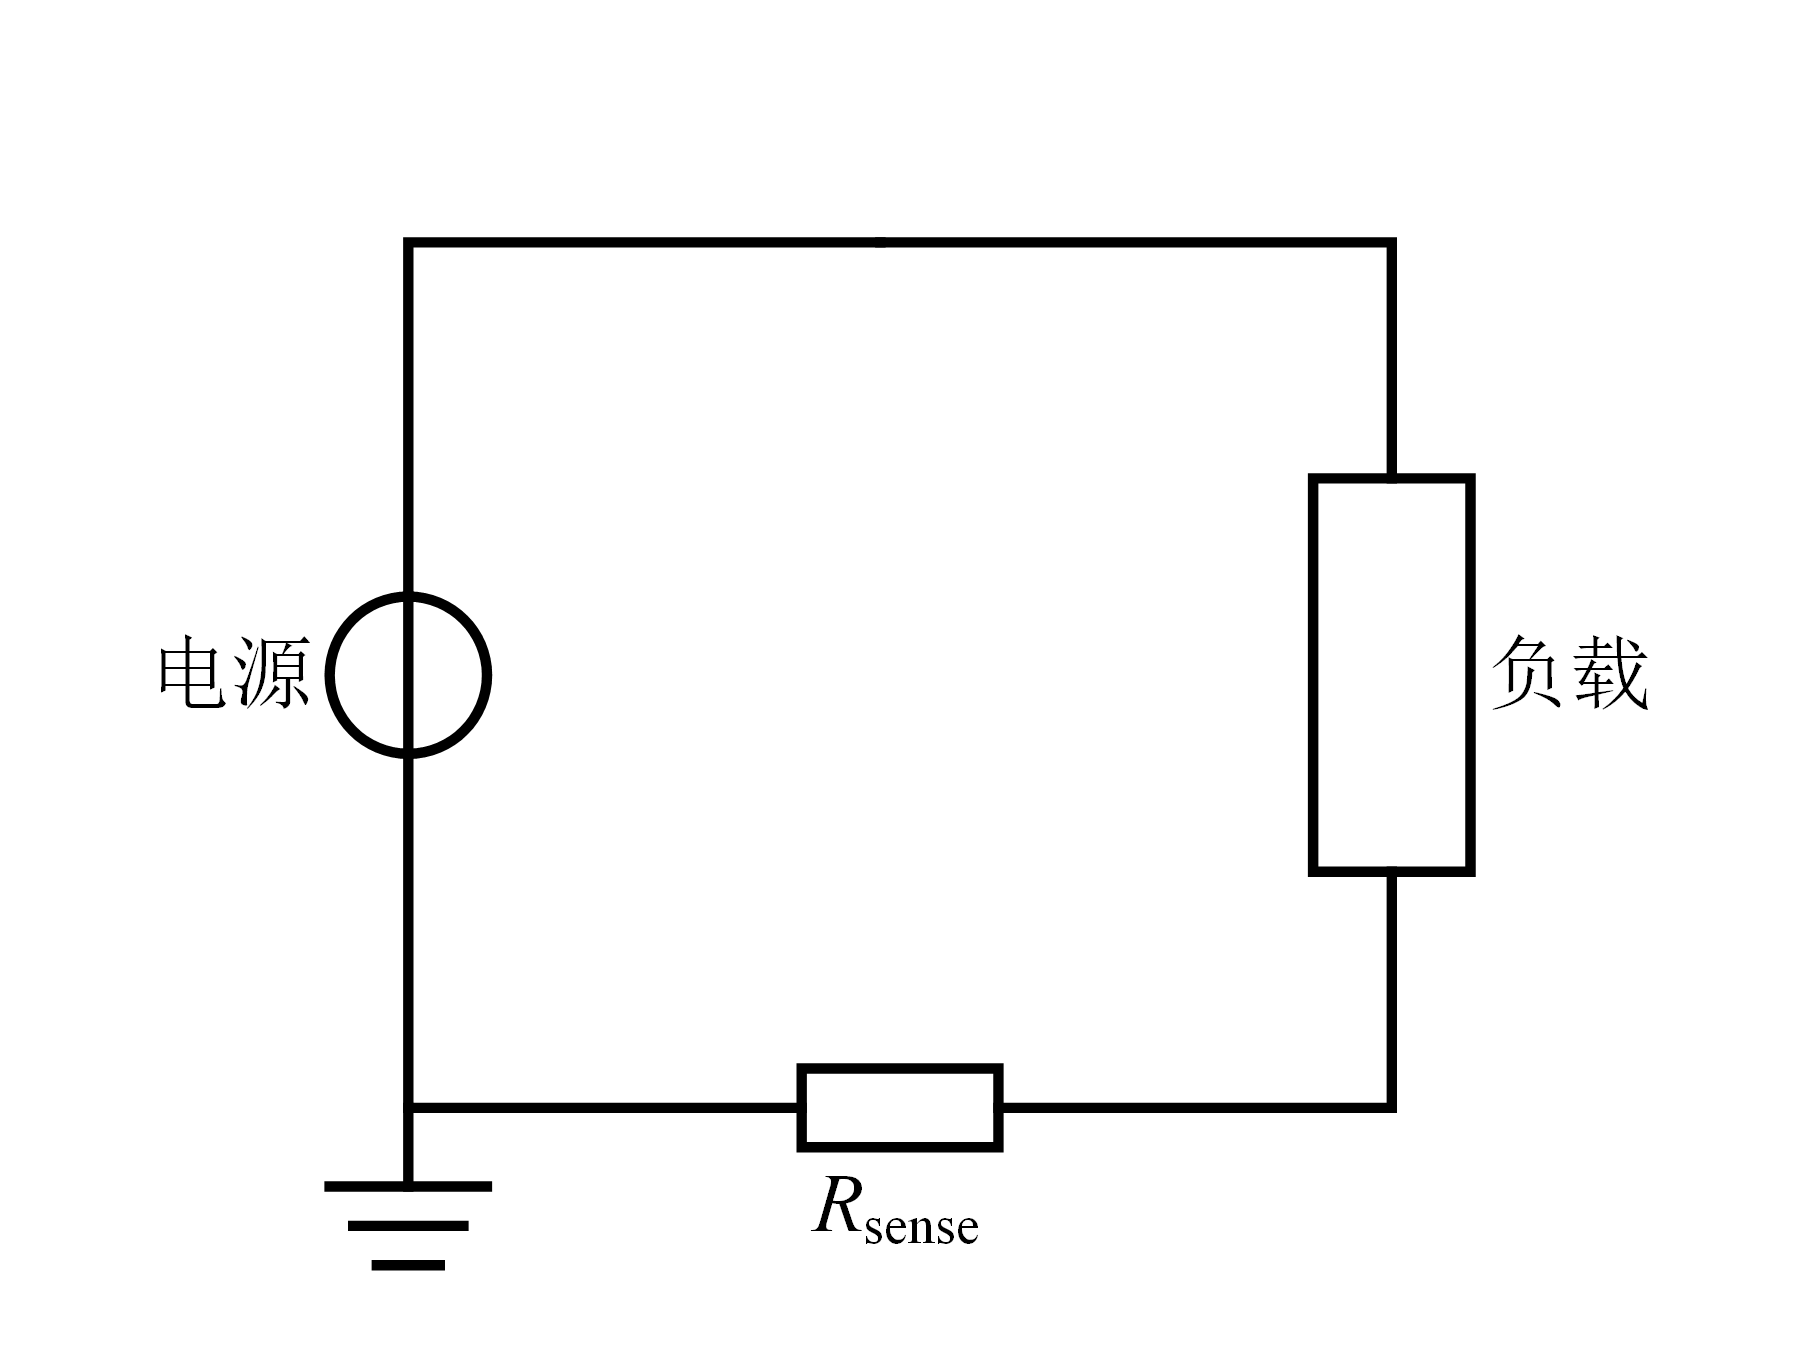
\includegraphics[scale=1.0]{picture/2_resistor_location_low.png}
            \label{f2.2:sf2}
        }
        \caption{采样电阻位置分布}
        \label{f2.2}
    \end{figure}

    1)高侧电流采样,采样电阻放置在电源和负载之间,输出电流先经过采样电阻,电阻下端对地至少为电源电压,具有较高的共模分量,对电路
    要求较高;

    2)低侧电流采样,采样电阻放置在负载和功率地之间,输出电流从负载流出,经过采样电阻回到功率地,电阻输出电压没有很高的共模分量,
    测量相对于高侧采样容易很多。

    两者的主要区别在于:

    1)因为采样电阻位置不同,引入了不同的共模分量,电路设计有一定差异。高侧电流采样要求后级信号调理电路具有较高的CMRR,后者则没有
    太多的要求。由于电阻失配、器件寄生参数等原因,CMRR参数一般在高频段时衰减得厉害,对高频干扰抑制能力下降很多。如果输出电压$V_
    {\rm out}$直接送到采样端,则高侧电流采样不适用于采样电阻具有较高噪声的场合,如MOS管电流采样、电机相电流采样,一般采用低侧电流
    采样。如果采用高侧电流采样,非常容易在$V_{\rm out}$上引入开关噪声。

    2)短路耐受能力,当负载对地短路时,高侧电流采样电阻需要承受全部的短路电流$I_{\rm short}$,此时电阻受到电流冲击而发热、甚至烧
    毁;而低侧电流采样电阻承受的短路电流由短路点位置决定,如果短路点在负载和低侧采样电阻之间,则采样电阻被短路,电阻承受较小的短路
    电流(短路点阻抗和采样电阻分流);若短路电在电源和负载之间,电阻上不留过任何短路电流。

    \begin{figure}[H]
        \centering
        \subfigure[高侧电流采样短路]{
            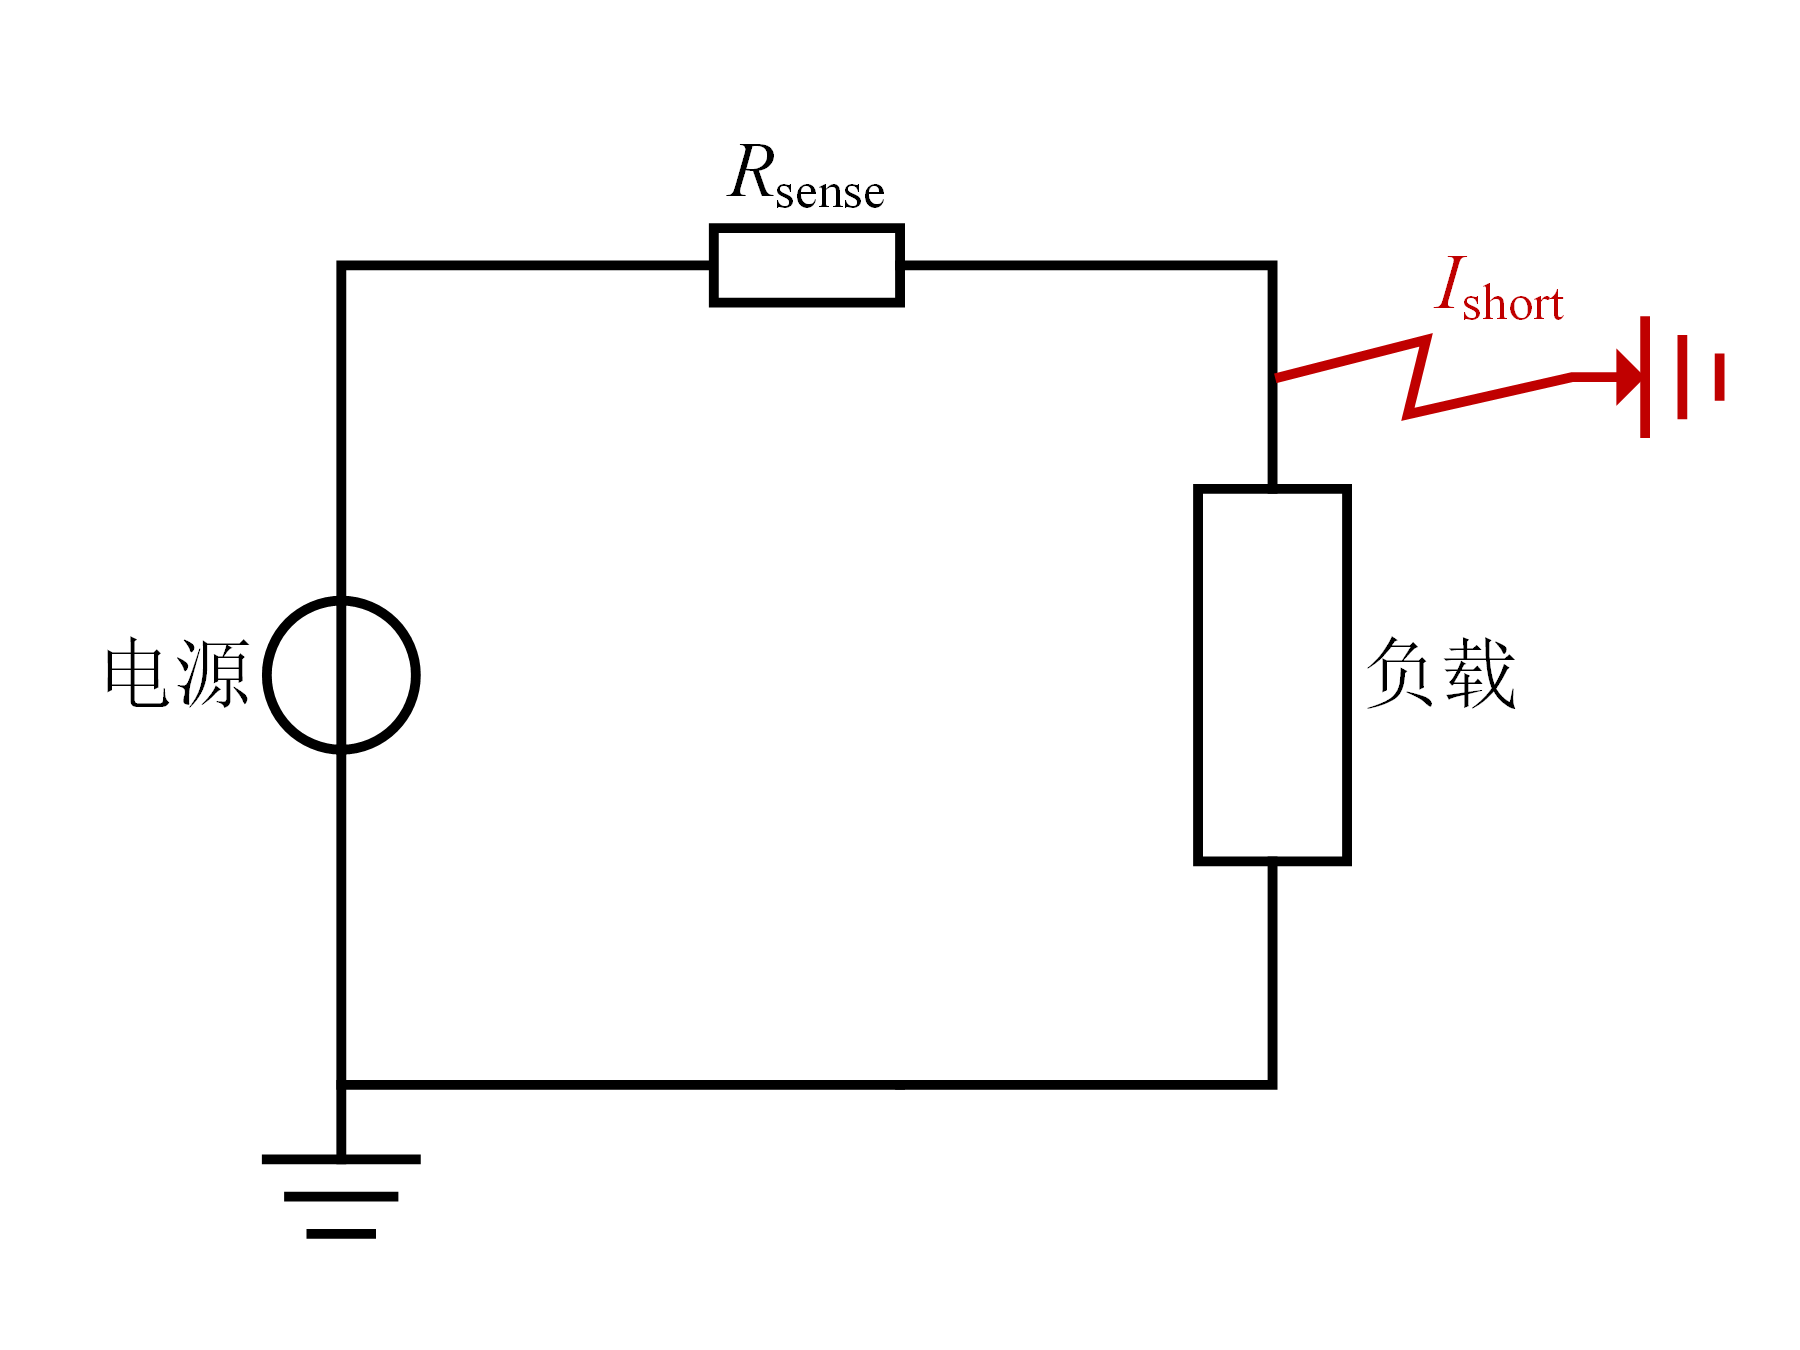
\includegraphics[scale=1.0]{picture/2_resistor_location_high_short.png}
            \label{f2.3:sf1}
        }
        \subfigure[低侧电流采样短路]{
            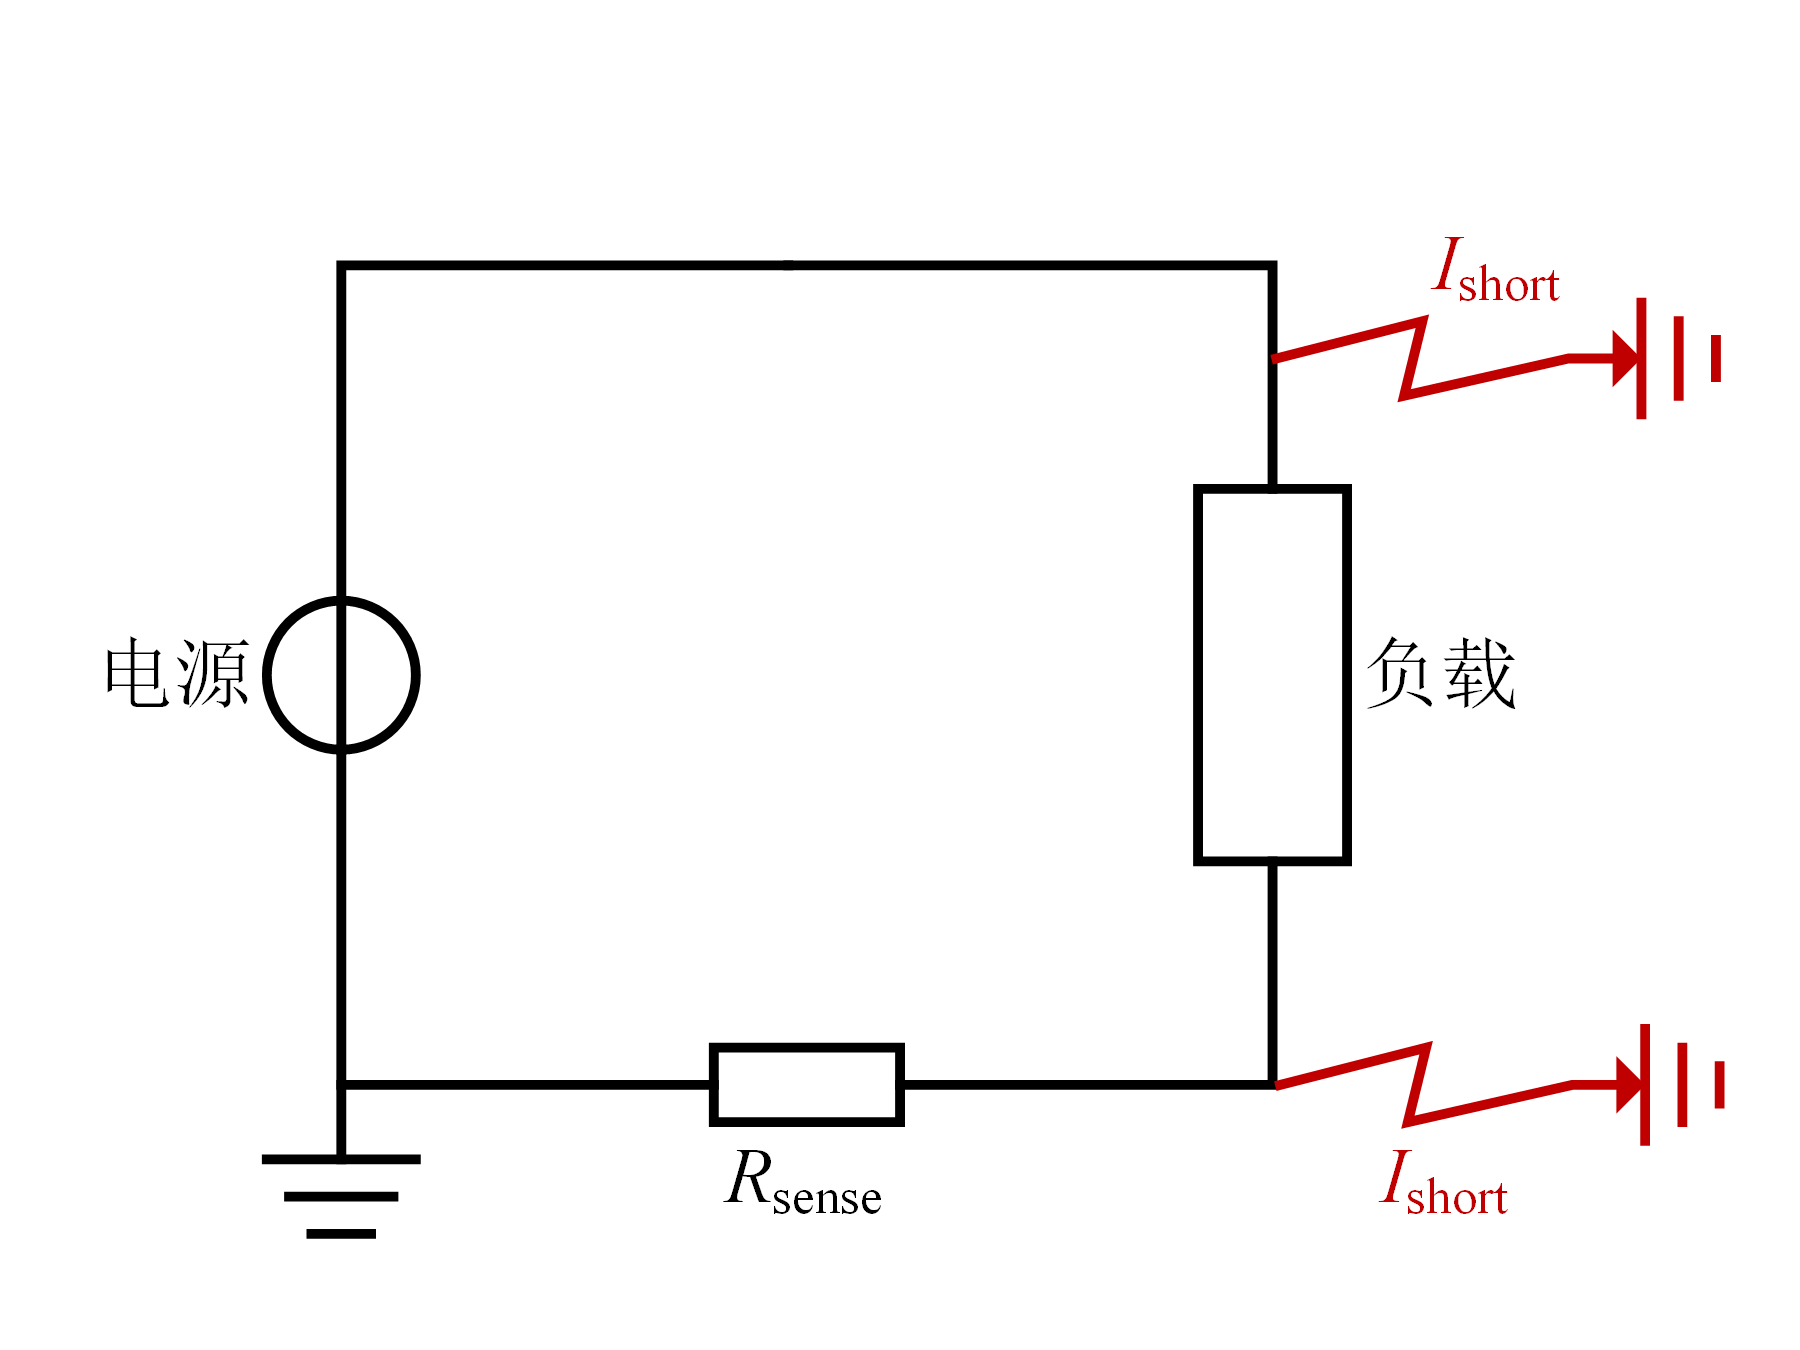
\includegraphics[scale=1.0]{picture/2_resistor_location_low_short.png}
            \label{f2.3:sf2}
        }
        \caption{不同采样电阻位置分布短路工况}
        \label{f2.3}
    \end{figure}
    
    3)故障情况检测能力,如第2点分析,高侧电流采样更容易检测出负载故障;而低侧电流采样则对于故障检测的能力较弱,如短路工况,不同
    短路点位置下流过采样电阻的故障电流不同,不容易判断。高侧电流采样可用于电池充放电流采样场合,故障检测能力更强。


% ===============================================第三章节=============================================== %
\section{器件特性}
    图\ref{f2.1}中包含多个电阻、电容原件以及运放元件,每个元件的特性都会对输出产生影响,下面对器件的特性进行分析,为后面的方案
    性能分析做准备。

\subsection{电阻特性}
    电阻的特性较为简单,除了常规的阻值、封装、最大允许功率耗散等特性外,还包含精度、温漂、稳定性、材质等其他特性,下面主要针对影
    响方案性能的因素进行分析。

    \subsubsection{电阻精度}
        电阻的精度一般指电阻的公差(Tolerance),

\subsection{运放特性}

\subsection{电容特性}

% ===============================================第四章节=============================================== %
\section{方案性能分析}
\subsection{传递函数分析}

\subsection{稳态特性分析}

\subsection{暂态特性分析}

\subsection{噪声特性分析}

% ===============================================第五章节=============================================== %
\section{设计实例}
\subsection{电路要求}

\subsection{需求拆解}

\subsection{理论设计}

\subsection{原理图设计}

\subsection{PCB设计}

\subsection{实物测试}

\subsection{测试与理论对比}

\end{document}